\documentclass{article}
\usepackage{comment}
\usepackage{float} %Imports biblatex package
\usepackage{multirow}
\usepackage{makecell}
\usepackage{graphicx}
\usepackage{subcaption}
\usepackage{caption}
\usepackage[square,numbers]{natbib}
\bibliographystyle{plainnat} %Citation-related commands

% if you need to pass options to natbib, use, e.g.:
% \PassOptionsToPackage{numbers, compress}{natbib}
% before loading neurips_2021

% ready for submission
%\usepackage{neurips_2021}

% to compile a preprint version, e.g., for submission to arXiv, add add the
% [preprint] option:
\usepackage[preprint]{neurips_2021}
% to compile a camera-ready version, add the [final] option, e.g.:
%     \usepackage[final]{neurips_2021}

% to avoid loading the natbib package, add option nonatbib:
%\usepackage[nonatbib]{neurips_2021}

\usepackage[utf8]{inputenc} % allow utf-8 input
\usepackage[T1]{fontenc}    % use 8-bit T1 fonts
\usepackage{hyperref}       % hyperlinks
\usepackage{url}            % simple URL typesetting
\usepackage{booktabs}       % professional-quality tables
\usepackage{amsfonts}       % blackboard math symbols
\usepackage{nicefrac}       % compact symbols for 1/2, etc.
\usepackage{microtype}      % microtypography
\usepackage{xcolor}         % colors

\title{
  Deep Learning Method For Predicting Nucleosome Positioning in Genomes using Genomic Signal Processing Techniques 
}

% The \author macro works with any number of authors. There are two commands
% used to separate the names and addresses of multiple authors: \And and \AND.
%
% Using \And between authors leaves it to LaTeX to determine where to break the
% lines. Using \AND forces a line break at that point. So, if LaTeX puts 3 of 4
% authors names on the first line, and the last on the second line, try using
% \AND instead of \And before the third author name.

\author{%
  Akshay Valsaraj \\
  BITS Pilani, K. K. Birla Goa Campus \\
  f20180608@goa.bits-pilani.ac.in
  \And
  Gourav Saha \\
  BITS Pilani, K. K. Birla Goa Campus \\
  f20180639@goa.bits-pilani.ac.in
  \And
  Ithihas Madala \\
  BITS Pilani, K. K. Birla Goa Campus \\
  f20180607@goa.bits-pilani.ac.in
  \And
  Prof. Sumit Biswas \\
  VISTA Lab \\ 
  Department of Biological Sciences \\
  BITS Pilani, K. K. Birla Goa Campus \\
  sumit@goa.bits-pilani.ac.in
  % examples of more authors
  % \And
  % Coauthor \\
  % Affiliation \\
  % Address \\
  % \texttt{email} \\
  % \AND
  % Coauthor \\
  % Affiliation \\
  % Address \\
  % \texttt{email} \\
  % \And
  % Coauthor \\
  % Affiliation \\
  % Address \\
  % \texttt{email} \\
  % \And
  % Coauthor \\
  % Affiliation \\
  % Address \\
  % \texttt{email} \\
}

\begin{document}

\maketitle

\begin{abstract}
Application of Digital Signal Processing techniques (DSP and DIP) to solve Genomics
problems initiated the new field Genomics Signal Processing (GSP) which concentrates to 
encode the Genomics signals based on DSP/DIP framework. In this Genomics era, high 
throughput DNA sequencing and the use of DNA microarray to simultaneously conduct 
huge number of experiments has lead to many signal/image processing problems. 
There is an emergent need to develop signal/image-processing techniques to examine 
data and determine relationship between genes. In this paper, we will focus on 
application of DSP and Machine Learning in Biomolecular Sequence Analysis.

\end{abstract}

\section{Introduction}
Genomic Signal Processing (GSP) is the processing, analysis and utilization of genomic signals to obtain relevant insights into the gene. This information is then used in the interpretation of particular gene motifs and families further resulting in the ability to classify diseases. DNA's critical role in all life's processes warrants its interpretation from different perspectives and interestingly, signal processing techniques reveal a better understanding. Over the recent years, GSP has captured researchers' attention because it allows quick analysis of genomic data with highly optimised coding for signal processing. Furthermore, this spectral data can easily be transformed into spectogram representations.

The nucleosome is considered the most basic unit of eukaryotic chromatin \citep{Richmond1038nature01595-ni}. The DNA is tightly packaged around the histone proteins under the action of regulatory proteins as well as recognised gene sequences \citep{Satchwell1986-ku}. The DNA packaged in the nucleosomes have regulated accessibility and play an important role in transcriptional control, DNA replication, DNA repair and RNA splicing etc. \citep{Berbenetz2010-09-02-hm}. We used a dataset containing DNA sequences that either promote or inhibit nucleosome formation to test the accuracy with which our model can differentiate between the two across multiple species.

\section{Methods}

\textbf{Datasets} \\ \\
In this article, we considered the following three species: 
(i) H.sapiens;(ii) C.elegans; and (iii) D.melanogaster.The data was obtained from 
\citep{Guo1093bioinformaticsbtu083-ss}.According to the paper, H.sapiens genome and its 
nucleosome map contains a hugeamount of data hence the  
nucleosome forming sequence samples (positive data) and the linkers or nucleosome inhibiting sequence samples (negative data) were 
extracted from chromosome 20. \\ \\
As for the other two species, namely C.elegans and D.melanogaster, 
the positive and negative data were extracted from their entire genomes. 
In the datasets thus formed from the three organisms, 
each of the DNA fragments was assigned with a nucleosome formation score to reflect its propensity to form nucleosome: the higher the score was, 
the more likely the fragment would be in forming a nucleosome. 
The DNA fragments with the highest nucleosome formation scores were selected as the nucleosomal sequences, while those with the lowest scores 
as the linker sequences. \\ \\
A dataset containing many redundant samples with high similarity would be lack of 
statistical representativeness. A predictor, if trained and tested by such a biased benchmark dataset, might yield misleading results with overestimated 
accuracy \citep{Chou1038nprot2007-xf}. To get rid of redundancy and avoid bias,
the CD-HIT software (Fu et al., 2012) was used with the cutoff threshold set at 80\% 
to remove those DNA fragments with high sequence similarity (note that the 
most stringent cutoff threshold for DNA sequences by CD-HIT was 75\%).


\begin{table}[h]
  \centering
  \begin{tabular}{|c|c|c|l}
  \cline{1-3}
  \begin{tabular}[c]{@{}c@{}}Species \\ type\end{tabular} &
    \begin{tabular}[c]{@{}c@{}}Nucleosome\\ forming\\ sequences\end{tabular} &
    \begin{tabular}[c]{@{}c@{}}Nucleosome\\ inhibiting\\ sequences\end{tabular} &
     \\ \cline{1-3}
  H.sapiens      & 2273 & 2300 &  \\ \cline{1-3}
  C.elegans      & 2567 & 2900 &  \\ \cline{1-3}
  D.mealnogaster & 2900 & 2850 &  \\ \cline{1-3}
  \end{tabular}
  \vspace{0.05in}
  \caption{Nucleosome forming and inhibiting sequences in the Three datasets used}
  \end{table}

\textbf{Converting DNA Sequence to Signal}\\
In order to apply signal processing techniques on gene sequences, there is a need to first convert the gene sequences from the nucleotides to more discrete numerical sequences. The latter can then be treated as digital signals. One of the most common ways used is to assign different numbers to each nucleotide and generating the signal. These mappings can either be fixed (that does not take any biological context) or they might be adaptive depending on adjacent nucleotides or thermodynamics properties. In general, there is no agreement on which representation makes the mos accurate signals. In our case, we use the tetrahedron representation in which each nucleotide corresponds to a vertex of a three-dimensional structure that is characterized by having equal distances between every pair of vertices \citep{Silverman1986-by}.


\textbf{Forming Spectrograms}\\
The DNA signal is used to develop spectrogram images for our model. N-point Discrete Fourier Transform (DFT) is first applied to the DNA signal after which Short Time Fourier Transform (STFT) is applied over a sliding window of 9 with an overlap of 6.The hamming function \citep{1455106}is used for the window to prevent spectral leakage. Once processed, colour spectrograms are defined by super imposing the three signals under the red, green and blue (RGB) values. The tetrahedron coefficients further increase the segregation of the sequences. In the spectrogram, the horizontal axis corresponds to the nucleotide number and the vertical axis refers to the discrete frequency of the DFT measured in the STFT cycles per window size. The spectogram was then resized to $224x224$ so that it could be used as an input for the deep learning model.
The tetrahedron coefficients used are : \\ \\
$ar = 0$,
$ag = 0$,
$ab = 1$,\\
$tr = 0.911$,
$tg = -0.244$,
$tb = -0.333$,\\
$cr = 0.244$,
$cg = 0.911$,
$cb = -0.333$,\\
$gr = -0.817$,
$gg = -0.800$,
$gb = 0$,\\

\begin{figure}[H]
  \centering
  \begin{subfigure}{4.6cm}
    \centering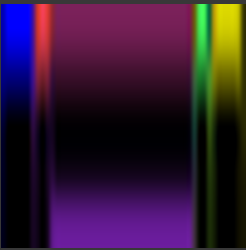
\includegraphics[width=4.6cm]{ATAT.png}
  \end{subfigure}
  \begin{subfigure}{4.6cm}
    \centering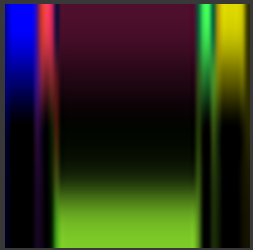
\includegraphics[width=4.6cm]{CGCG.png}
  \end{subfigure}
  \begin{subfigure}{4.6cm}
    \centering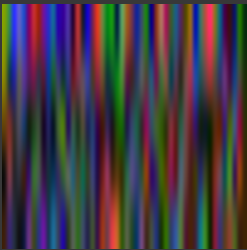
\includegraphics[width=4.6cm]{sequence.png}
  \end{subfigure}
  \caption{ \textbf{Left}:Spectrogram of DNA of length 147bp with bases A, T, C, and G , respectively. The nucleotide A is represented by the color blue, T by red, C by green, and G by yellow.The interaction between the various nucleotides is visualized as the superposition of colors representing those nucleotides.
  This represents the sequence having AT repeat in between,  the purple is due to a superposition of red and blue from A and T. \\
  \textbf{Center} : This represents the sequence having CG repeat in between,  the greenish yellow is due to a superposition of yellow and green from G and C.\\
  \textbf{Right}: A spectogram of a sequence taken from the dataset.}
  \label{fig:ROC}
\end{figure}

\textbf{Model}\\
To train the model we used the densenet architecture \citep{huang2018densely}.DenseNet-121 consists of 121 densely connected convolutional layers with a fully conncted(FC) layer of 1000 units as its final output layer. We removed the final layer and replaced it with a FC layer with two neurons for two class classification.

\begin{figure}[H]
  \centering
  \begin{subfigure}{10.5cm}
    \centering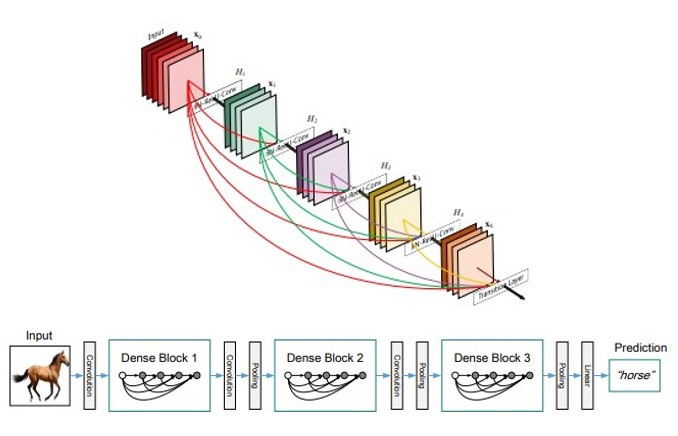
\includegraphics[width=10.5cm]{densenet.jpeg}
  \end{subfigure}
  \caption{A deep DenseNet with three dense blocks. The layers between two adjacent blocks are referred to as transition layers and change
feature-map sizes via convolution and pooling.}
 \label{fig:previous_results}
\end{figure}
\section{Results}
We present 2 types of results ,For the first type of results we wanted to know how well the pattern of the data could be reflected with different species so we 
trained on two different species and tested on the third and this was done for all the species. \citep{Guo1093bioinformaticsbtu083-ss} had done a 
one-vs-All classification results where they trained a model on N-1 sequences and tested it on one of the classes and this was done N times to generate the class for each sequence individually , since this would be very memory intensive we didn't go for this approach. \\ 
The second type of results we combined all the 15498 sequences and divided it into 12553 train sequences, 1395 validation sequences and 1550 test sequenences. 
In the test sequence 457 sequences belonged to H.sapiens,518 to C.elegans and 575 to D.mealnogaster. \\
Moreover in the test results we made sure to show the results for each species separately so that we could compare it with the previous results obtained by  \citep{Guo1093bioinformaticsbtu083-ss}.

\textbf{Type 1 Results} \\
In this case we trained on two species and tested on the third. For example for H.sapiens we trained on C.elegans and D.mealnogaster
and tested on  H.sapiens. \\

\begin{figure}[]
  \centering
  \begin{subfigure}{4.6cm}
    \centering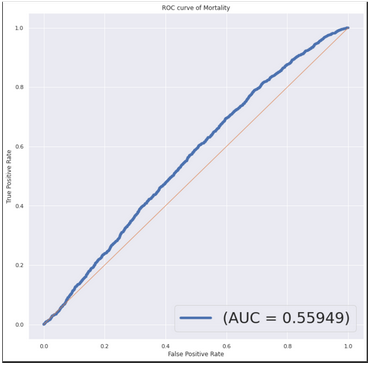
\includegraphics[width=4.6cm]{C_elegans.png}
  \end{subfigure}
  \begin{subfigure}{4.6cm}
    \centering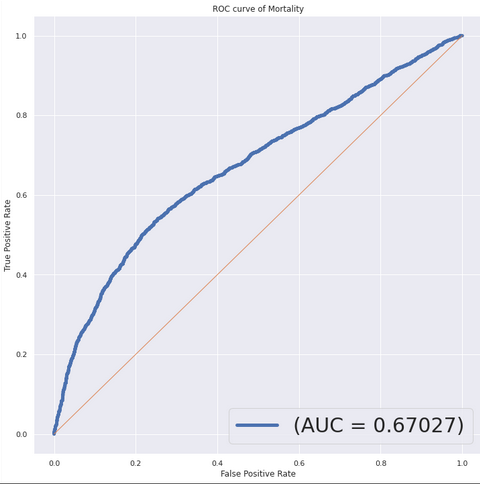
\includegraphics[width=4.6cm]{D.mealnogaster.png}
  \end{subfigure}
  \begin{subfigure}{4.6cm}
    \centering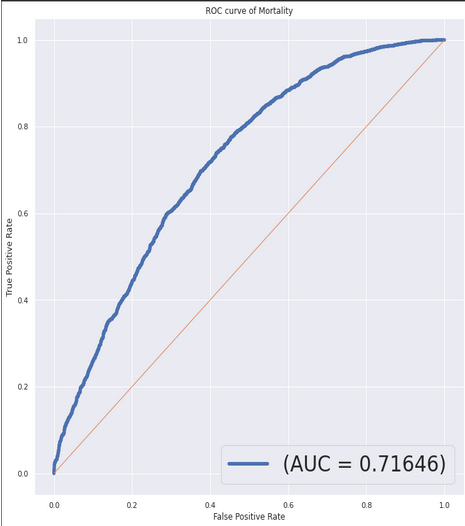
\includegraphics[width=4.6cm]{sapiens.png}
  \end{subfigure}
  \caption{ 
  \textbf{Left}:ROC curves for  C.elegans.
  \textbf{Center} : ROC curves for  D.mealnogaster.
  \textbf{Right}: ROC curves for  H.sapiens.}
  \label{fig:ROC}
\end{figure}

\begin{figure}[]
  \centering
  \begin{subfigure}{4.6cm}
    \centering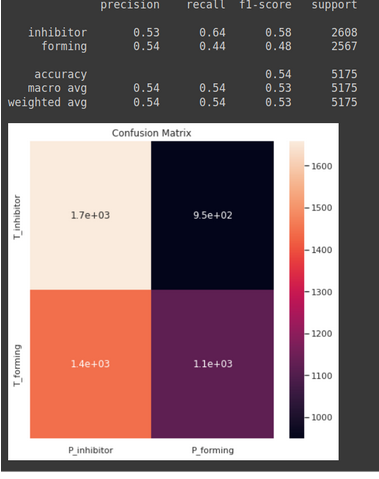
\includegraphics[width=4.6cm]{C_elegans_cm.png}
  \end{subfigure}
  \begin{subfigure}{4.6cm}
    \centering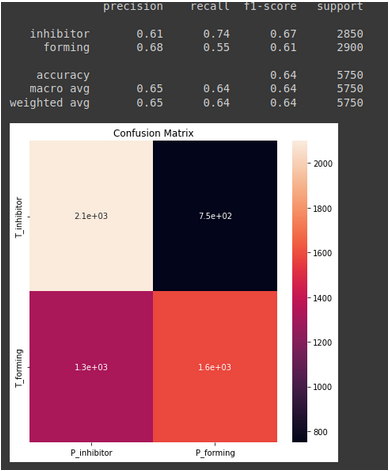
\includegraphics[width=4.6cm]{D.mealnogaster_cm.png}
  \end{subfigure}
  \begin{subfigure}{4.6cm}
    \centering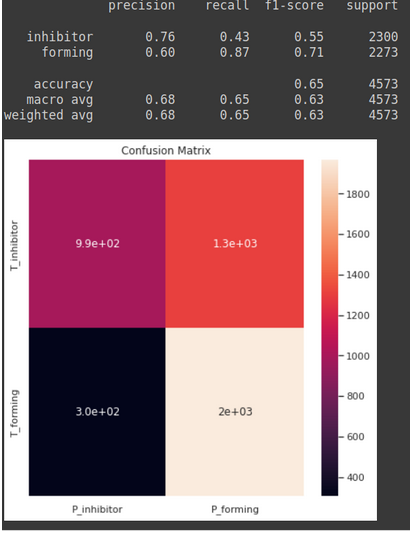
\includegraphics[width=4.6cm]{sapiens_cm.png}
  \end{subfigure}
  \caption{ 
  \textbf{Left}:Confusion Matrix for  C.elegans.
  \textbf{Center} : Confusion Matrix for  D.mealnogaster.
  \textbf{Right}:Confusion Matrix for  H.sapiens.}
  \label{fig:Confusion_matrix}
\end{figure}

\textbf{Type 2 Results} \\
In this case we trained on 12553 train sequences with 1395 as validation sequences and predicted on 1550 test sequences.\\


\begin{figure}[]
  \centering
  \begin{subfigure}{4.6cm}
    \centering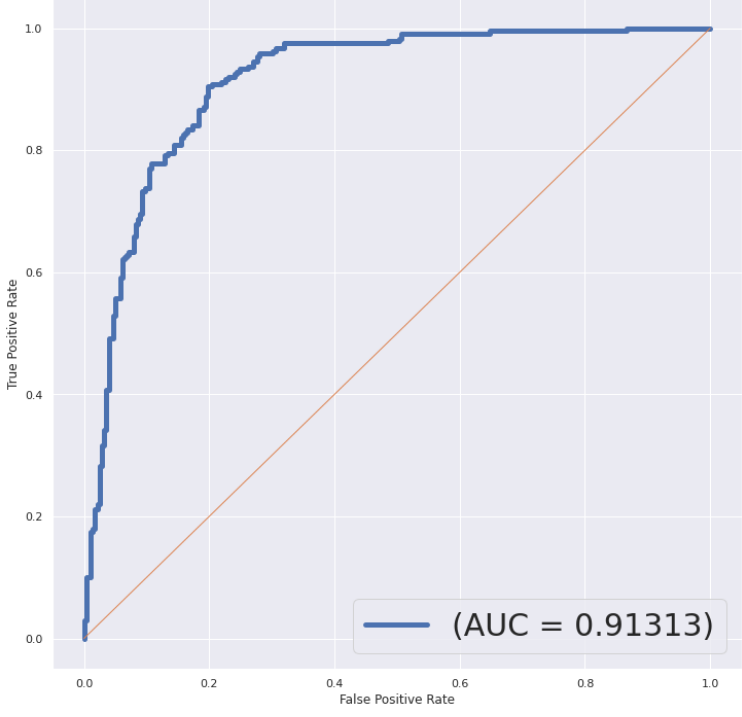
\includegraphics[width=4.6cm]{C_elegans_all_roc.png}
  \end{subfigure}
  \begin{subfigure}{4.6cm}
    \centering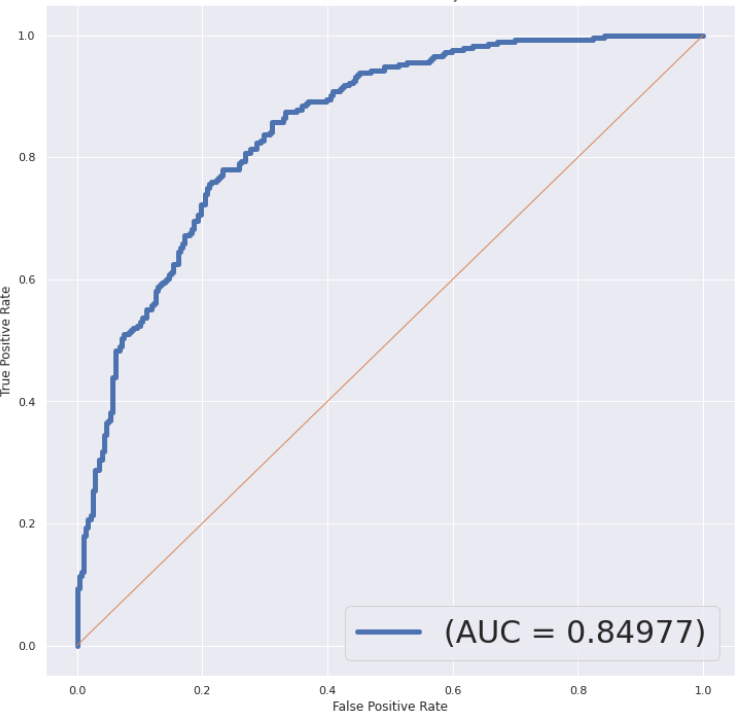
\includegraphics[width=4.6cm]{D.mealnogaster_all_roc.png}
  \end{subfigure}
  \begin{subfigure}{4.6cm}
    \centering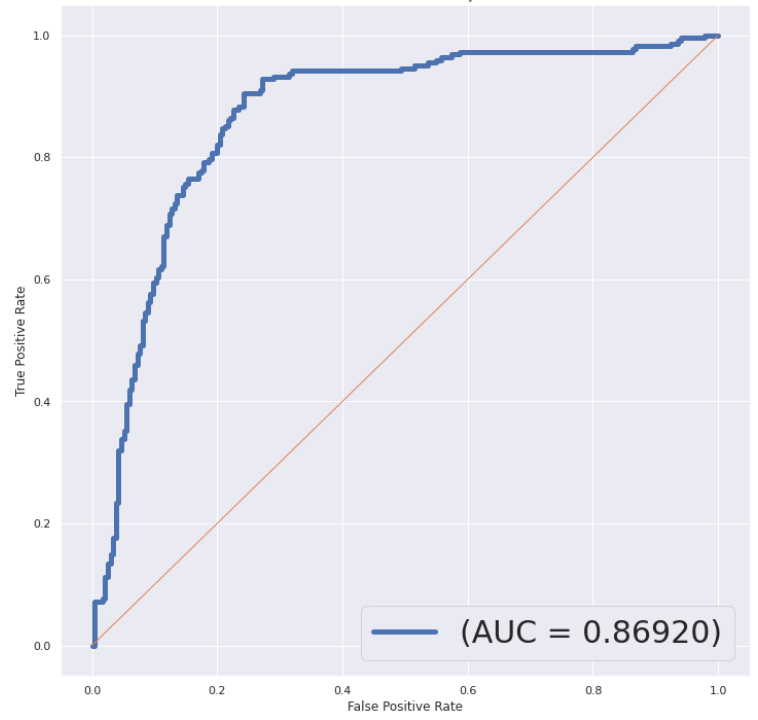
\includegraphics[width=4.6cm]{sapiens_all_roc.png}
  \end{subfigure}
  \caption{ 
  \textbf{Left}:ROC curves for  C.elegans.
  \textbf{Center} : ROC curves for  D.mealnogaster.
  \textbf{Right}: ROC curves for  H.sapiens.}
  \label{fig:ROC_all}
\end{figure}

\begin{figure}[]
  \centering
  \begin{subfigure}{4.6cm}
    \centering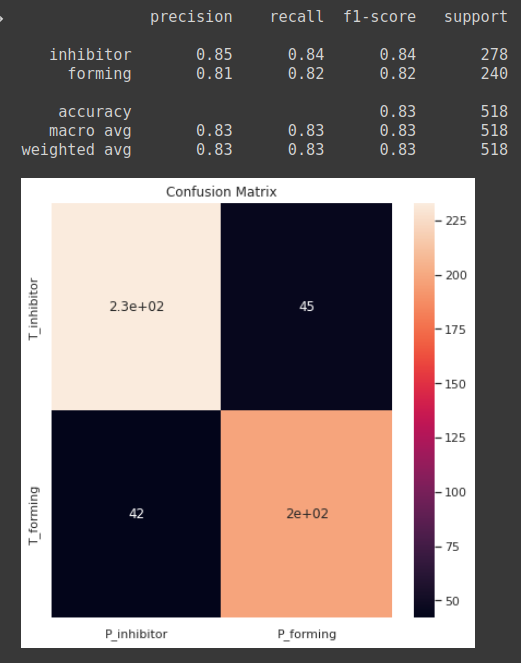
\includegraphics[width=4.6cm]{C_elegans_all_cm.png}
  \end{subfigure}
  \begin{subfigure}{4.6cm}
    \centering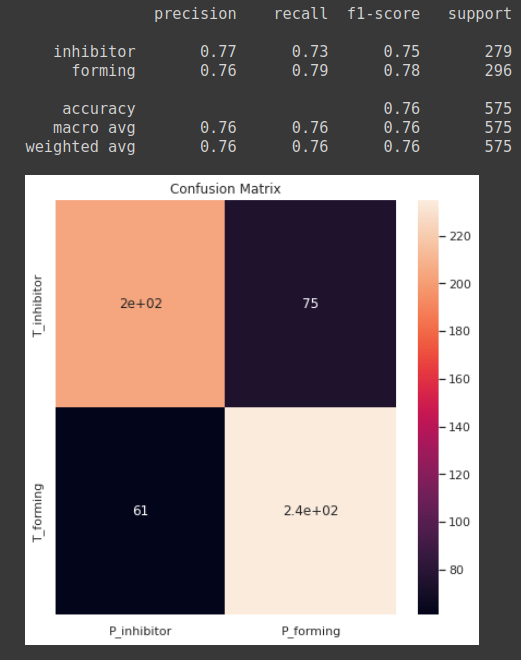
\includegraphics[width=4.6cm]{D.mealnogaster_all_cm.png}
  \end{subfigure}
  \begin{subfigure}{4.6cm}
    \centering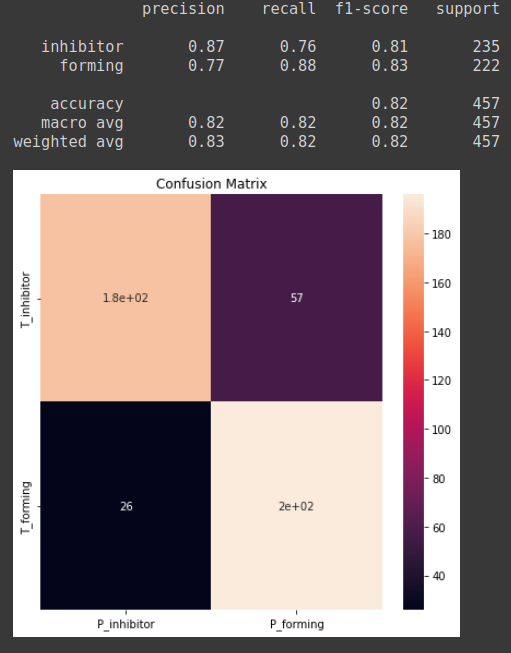
\includegraphics[width=4.6cm]{sapiens_all_cm.png}
  \end{subfigure}
  \caption{ 
  \textbf{Left}:Confusion Matrix for  C.elegans.
  \textbf{Center} : Confusion Matrix for  D.mealnogaster.
  \textbf{Right}: Confusion Matrix for  H.sapiens.}
  \label{fig:cm_all}
\end{figure}

\section{Conclusion}
\begin{figure}[H]
  \centering
  \begin{subfigure}{5.5cm}
    \centering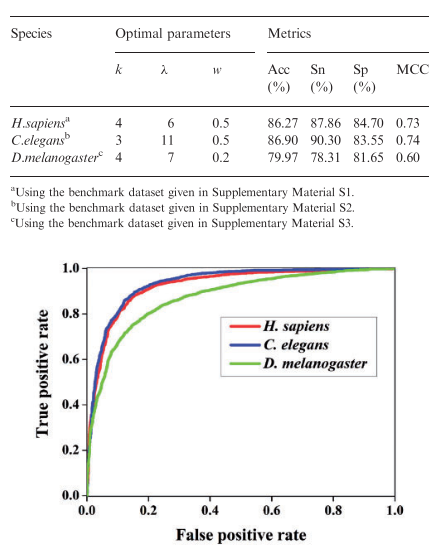
\includegraphics[width=5.5cm]{previous_results.png}
  \end{subfigure}
  \caption{A graphical illustration to show the performance of the iNuc- PseKNC by means of the ROC curves. The areas under the ROC curves, or AUROC, are 0.925, 0.935 and 0.874 for H.sapiens, C.elegans and D.melanogaster,respectively
  binary}
 \label{fig:previous_results}
\end{figure}

From \ref{fig:previous_results} we can see that we have come close to the results mentioned in the previous paper but we cannot take these as the benchmark as :
\begin{enumerate}
  \item \citep{Guo1093bioinformaticsbtu083-ss} has used a one vs all cross validation which uses all the data except one whereas was our results are only based on 80\% of the sequences which it has been trained on.
  \item Compared to previous works we have also presented the results of the model when it is tested on species trained on different species which would prevent similar sequences from the same species providing biases in the data.This could form as the benchmark for future research.
\end{enumerate}

\bibliography{references}


\end{document} 
